%!TEX root = ../thesis.tex

\cleardoublepage
\chapter{Example of Custom GTP Header Format}
\label{cha:qagent_example}

This appendix contains a screenshot of a packet trace displayed using wireshark \footnote{https://www.wireshark.org/}. The packet dissection shows the GTP format being used, along with the additional custom header, which is 8 bytes long. Consisting of 2 bytes of regular overhead from the protocol as wel as a 4 byte timestamp and 2 spare bytes.

\begin{figure}[ht]
    \centering
	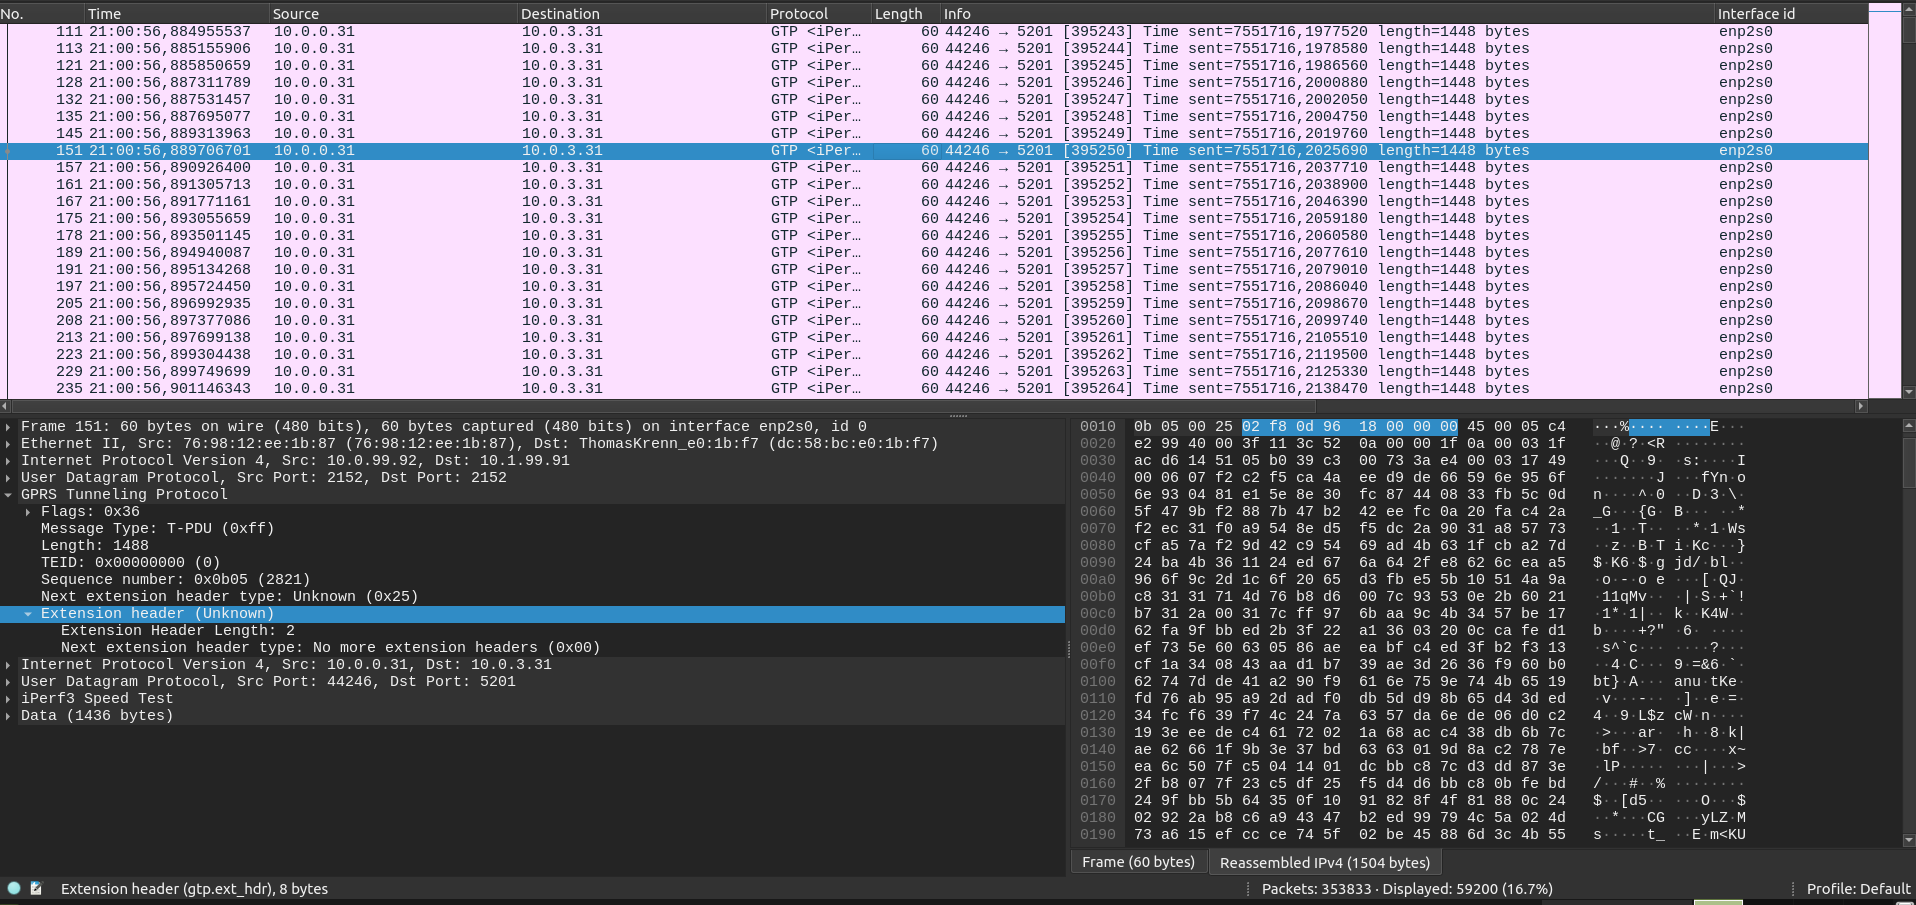
\includegraphics[width=\textwidth]{fig/gtp_packet.png}
	\caption{Screenshot of Wireshark Dissection Displaying the Custom Header Format}
	\label{fig:wshark}
\end{figure} 
